\chapter{Background and Related Work}
This chapter starts by first surveying related wearable devices for healthcare applications that are available on the market today.
We describe technical challenges that may be faced by developers in developing and prototyping wearable devices.
Second, we describe our own case study of building a wearable device from scratch without using any platform/tool support.
We detail the amount of development effort and skill needed to motivate the need for wearable platform \& tool support.
Third, we present related application development platforms and tools in which designers and developers can use to build their devices \& applications.
We describe how BioScope addresses the issues of flexibility and extendibility lacking from these related platforms \& tools.

\section{Wearable Devices with Healthcare Applications}
Recently, there have been many commercial products leveraging mobile sensing and wearable technologies to promote health in people's daily life. As smartphones become ubiquitous in people's daily life, people have explored the use of smartphones together with their built-in sensors to monitor human health condition, such as basic vital-signs. For example, Instant Heart Rate \cite{Instant_Heart_Rate} is a phone application that leverages the smartphone's built-in camera and flashlight to sense a person's heart rate. Strava \cite{Strava} is a smartphone application that uses the smartphone's GPS sensor to quantify human performance of running and cycling exercises. When built-in sensors are insufficient, smartphones can also connect with external sensors, such as wearable heart rate sensors and/or cycling sensors, to collect more detailed information for further analysis of the exercise events.

Wearable devices are not only an extension of a smartphone. They can also work as a standalone device. Being wearable, it reduces people's burden of carrying additional devices. In recent years, a variety of wearable products have successfully immersed in people's daily life. Wristband is the most common form factor in wearable devices. For example, the Fitbit \cite{Fitbit} is a popular wristband device that enables people to track and monitor their physical activities. The Apple watch \cite{Apple_watch} and the Android wear \cite{Android_wear} provide wearable computing platforms to build wearable healthcare applications in the wristband form factor. Other non-wristband wearable form factors are also emerging. For examples, the Under Armour \cite{Under_armour} releases a sensor-embedded running shoe that can track and collect running metrics. The Athos \cite{Athos} is a smart apparel that monitors muscle activities and heart rate to assist training and exercise. X2 xGuard \cite{X2_xGuard, camarillo2013head} is a product that embeds sensors inside a mouth guard for tracking athletes' accumulative head impacts in contact sports, e.g.: football. The forecast for wearable devices worldwide from Gartner \cite{gartner2016wearable} shows that the market of wearable healthcare devices will experience rapid growth in the near future. 

%[What are the technical challenges these devices face that you want to put in your platform?] 

Since wearable devices are deployed and worn on humans constantly, usability plays a particularly important factor to successful people's acceptance and adoption of wearable technologies. Reaching usability goal is costly, requiring designers and/or developers to perform many iterations of prototyping, testing, analyzing, and refining to uncover and fix problems. Such development and prototyping effort can be reduced with platform support. 
%[hardware] [software]

%\section{Rapid Prototyping in HCI}
%[tool for UI]
%[3D printing]
%[]
%A proper mechanism of rapid prototyping is always an critical factor to significantly affect the progress of entire design process. Therefore, 
%some HCI researchers have paid their attention to develop better rapid prototyping .
%For example, 

\section{Case Study of Developing a Wearable Device: Sensor-Embedded Teeth for Oral Activity Recognition}
This section presents a case study that we experienced the design and implementation of a wearable oral sensory system that recognizes human oral activities, such as chewing, drinking, speaking, and coughing from scratch without using any platform/tool support. 

\subsection{Motivation}
The human mouth is one part of the human body that is almost always in constant use. We use our mouth to perform some of the most important daily functions, such as eating, drinking, speaking, coughing, breathing, and smoking. Because our mouth is an opening into assessing the health of the human body, it presents the opportunity for the placement of a strategic sensor for detecting human oral activities. For this study, we developed such an oral sensory system, where we explored the use of a small motion sensor embedded inside artificial teeth for the recognition of human oral activities. The detection of human oral activities can enable numerous health care applications, such as food and fluid intake monitoring.   

%Previous research has explored wearable sensory devices installed in various locations of the upper body for detecting human oral activities. For example, Amft et al. \cite{Amft:2005} used an earphone-attached microphone sensor to record human chewing sounds and detect food types based on their acoustic profiles. Amft et al. \cite{Amft:pervasive2009} proposed another approach that combined surface Electromyography (EMG) and a microphone worn around the neck area to recognize low- or high-volume swallowing actions. BodyScope \cite{Yatani:2012} placed an acoustic sensor around the neck area to recognize different oral activities (e.g., eating, drinking, speaking, laughing, and coughing) by analyzing sounds generated from the throat area. In comparison, our oral sensory system explores a unique sensor placement not on the human body, but inside the human body, specifically the mouth. Because a sensor placement inside the mouth has the advantage of being in proximity to where oral activities actually occur, this enables our oral sensory system to accurately capture the motion of oral activities. 

This study presents the design and evaluation of this in-mouth oral sensory system, which uses a small accelerometer sensor embedded inside artificial teeth. Our motivation was based on our observation that most oral activities, such as chewing, drinking, speaking, and coughing, each produce a unique teeth motion. By recording and identifying teeth motion profiles for each oral activity, the proposed oral sensory system builds classifiers that distinguish different human oral activities. 

%The main contributions of this work are as follows: (a) We introduce an in-mouth, motion-based oral sensory system for detecting human oral activities; and (b) We conducted a laboratory experiment with 8 participants performing four common oral activities, which are chewing, drinking, speaking, and coughing. The results demonstrated the feasibility of this oral sensory system, in which a person-dependent classifier achieved 93.8\% recognition accuracy, and a person-independent classifier achieved 59.8\% accuracy.



\begin{figure}[!ht]
\centering
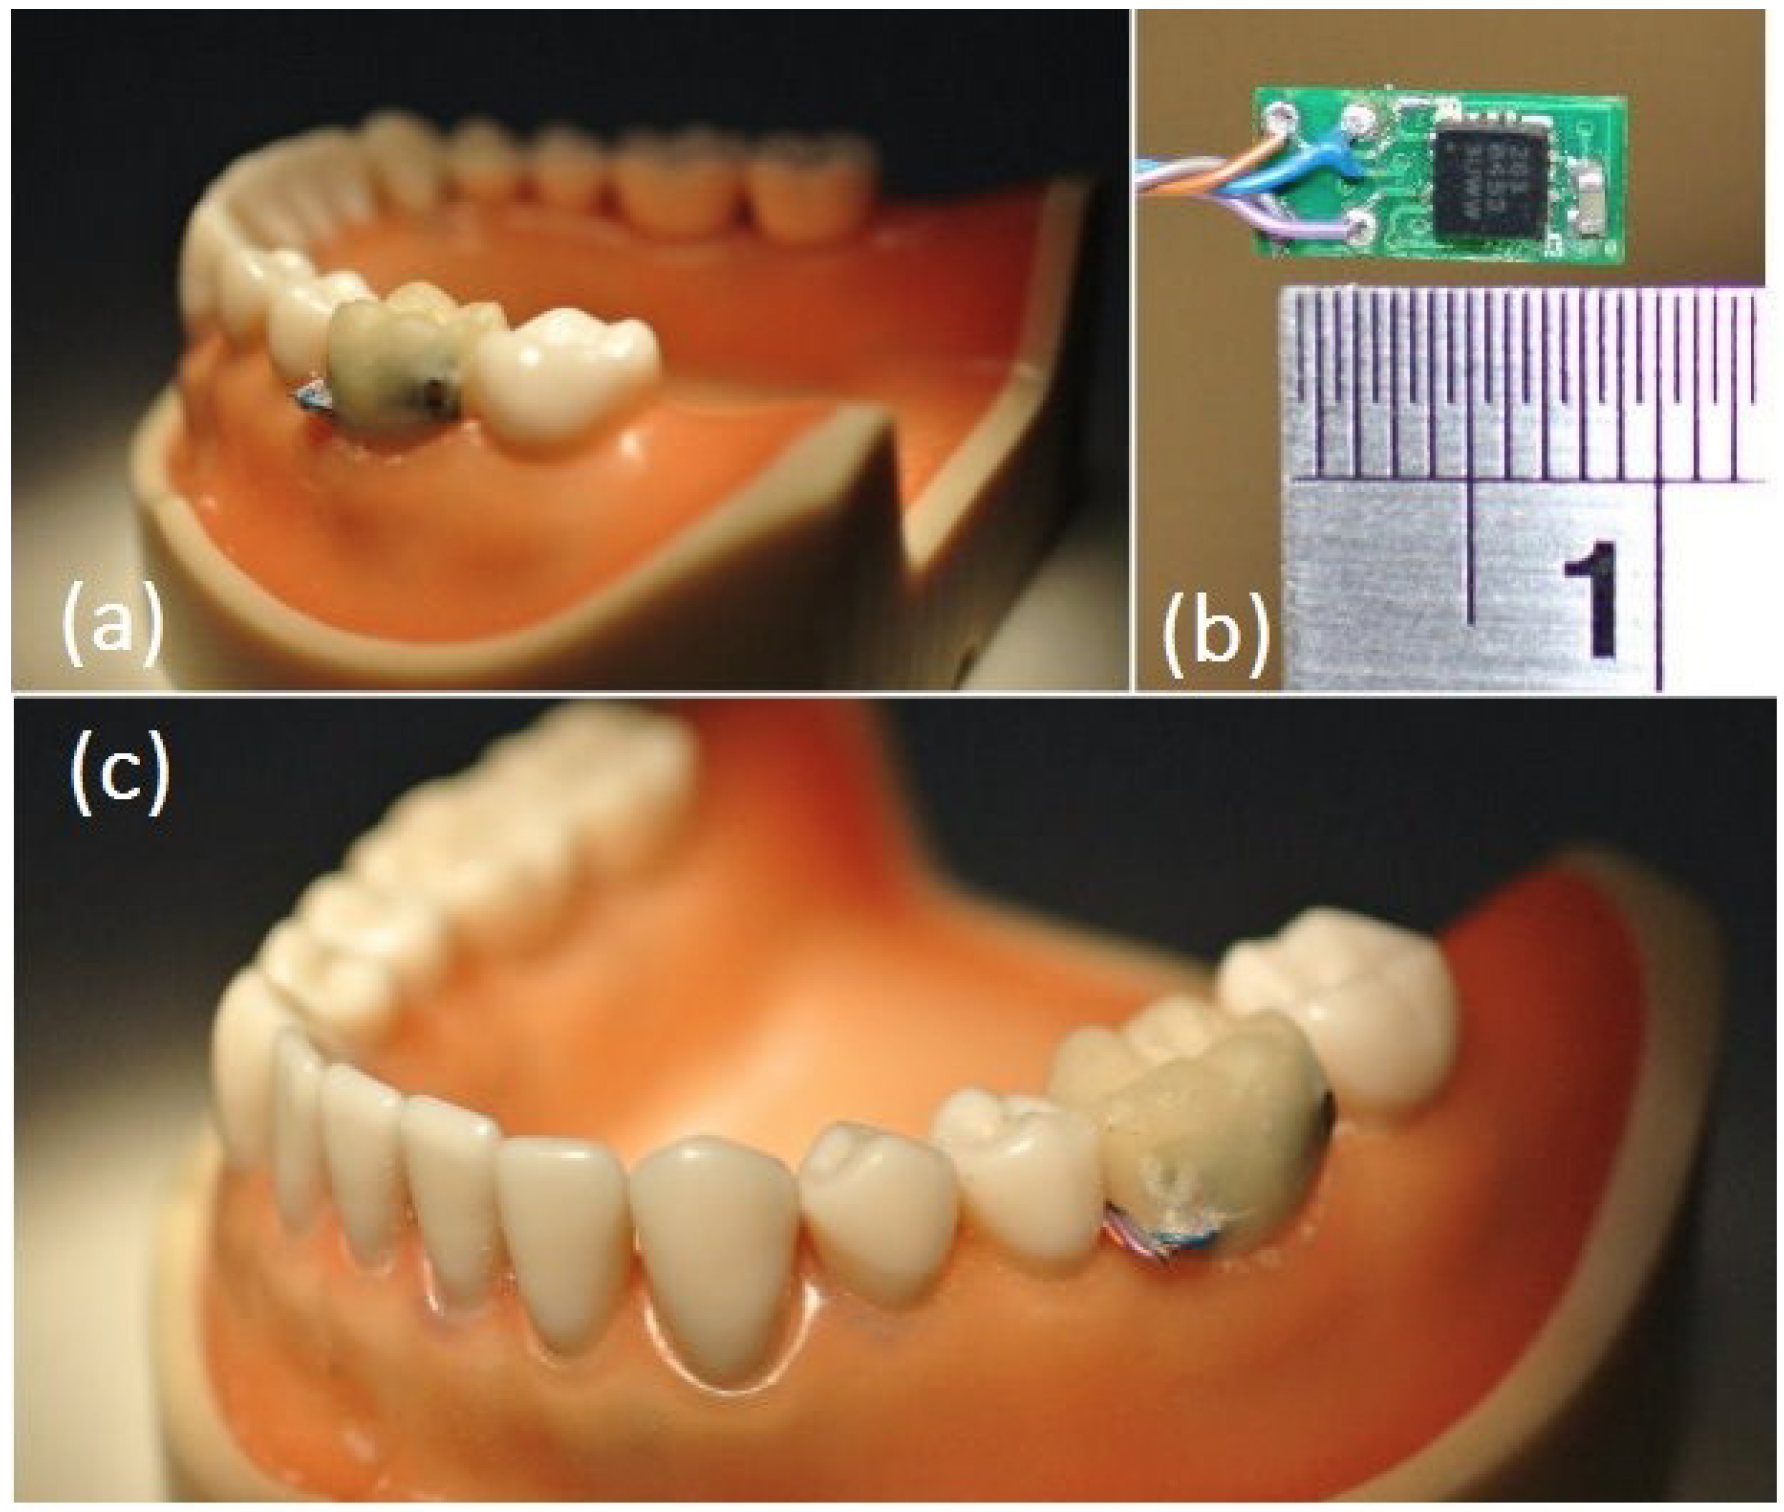
\includegraphics[width=14cm]{image/teeth.png}
\caption{The breakout board with (b) tri-axial accelerometer and (a)(c) sensor embedded denture.}
\label{teeth_overview}
\end{figure}


%\subsection{System Overview}
%The system consists of two main components: (a) an oral sensory unit; and (b) oral activity classifiers. 

\subsection{Oral Sensory Unit}
Figure \ref{teeth_overview}(b) shows a small breakout board with a tri-axial accelerometer sized 4.5 mm x 10 mm. This small breakout board is sufficiently small to be embedded inside a removable artificial tooth, as shown in Figure \ref{teeth_overview}(a) andFigure \ref{teeth_overview}(c). To ensure that this sensor board is safe and saliva-proof for human mouth placement, we carefully coated the sensor board with dental resin. In actual system deployment, this sensor board would include a small Bluetooth radio capable of wirelessly transmitting sensor data to a nearby mobile phone for data analysis and oral activity recognition. In the current proof-of-concept system, we have yet to place a Bluetooth radio on this oral sensory unit; therefore, thin wires are used to connect the sensor board to an external data-logging device for data retrieval and power. These thin wires also protect users from accidentally swallowing the sensor units.

\subsubsection{Oral Activity Analysis}
Oral activity recognition comprises the following three steps: (1) data preprocessing, (2) feature extraction, and (3) data classification. These steps are described as follows: 
\vspace{15pt}
\newline 
\textsl{\textbf{Data preprocessing:}}
\newline
The sampling rate of the accelerometer sensor is set to 100 Hz. The system first divides the accelerometer data into windows of 256 samples with a 50\% overlap between consecutive windows [4]. In each data window, the system extracts the time-domain and frequency-domain features shown in Table 2. 
Because people have different mouth and teeth specifications, sensor orientation can change for different users. Thus, accelerometer readings must be adjusted and calibrated using a rotation matrix. During the calibration phase, the proposed system asks users to hold their head straight and still for a few seconds during the application of Rodrigues' rotation formula to compute this rotation matrix. Each oral sensor unit has its own rotation matrix, which is used to transform its sensor readings from the device's coordinates to real-world coordinates. This normalization procedure reduces the negative effect of errors caused by varying device orientation. Because this normalization procedure reduces, but does not completely remove this error, the system also extracts orientation-independent features based on the magnitudes of x-, y-, and z-axis acceleration. For each sample at time t, its magnitude data is calculated as $\sqrt{x_{t}^{2}+y_{t}^{2}+z_{t}^{2}}$.


The normalized (orientation-dependent) feature set and the orientation-independent feature set have different characteristics. The normalized feature set retains separate information on tri-axial acceleration values, which are required for distinguishing activities involving both vertical and horizontal movements. In contrast, the orientation-independent feature set is based on the magnitude value, in which its precision is less affected by changes in device orientation; thus, it is suitable for distinguishing activities that depend on the movement scale.

\textsl{\textbf{Feature extraction:}}
We extracted the time-domain and frequency-domain features from each data window. Frequency-domain features are computed using the FFT algorithm. Both real and imaginary components of FFT coefficients in the 256-sample window are used to generate 256 features. Overall, the system trains activity classifiers by computing and extracting the following two feature sets: 807 features (269 features per axis acceleration) from the normalized feature set, and 269 features from the device-independent feature set.


\textsl{\textbf{Training Classifiers:}}
Our system implements three classifiers: the C4.5 Decision Three (DT), the Multivariate Logistic Regression (MLR), and the Support Vector Machine (SVM). The SVM classifier uses the radial basis function kernel and one-against-one multiclass classification, and it is further optimized by an additional parameter selection and data scaling. To filter out redundant and irrelevant features, we performed feature selection based on the correlations between features. Low-relevance features with low correlation are filtered out. We adopted principal component analysis [5] as a feature selector, in which the number of relevant features was reduced to 137. 
For each classification algorithm of the DT, the MLR, and the SVM, we trained two classifiers: person-dependent and person-independent. A person-dependent classifier uses data from all users (i.e., 8 participants in our study) to train a generalized activity model for recognizing the oral activities of different users. Conversely, a person-independent classifier uses 7 users' data to train a specify activity model for recognizing remaining person's oral activities.

\textsl{\textbf{Experiment results:}}
Eight users (5 males and 3 females) participated in this experiment. They were asked to install the oral sensor unit inside their mouth while performing each of these four oral activities: chewing, drinking, talking, and coughing. Because it was not possible to customize a removable tooth for each participant, we used dental cement to fix the sensor units to each participant's tooth.
We conducted 10-fold cross-validation and leave-one-person-out cross-validation to measure the accuracies of the person-dependent and person-independent classifiers. For the person-dependent classifiers, each round of cross-validation involved using all of each participant's data for both training and testing. Table 2 shows the mean F-measure accuracy results. The SVM (93.8\%) classifier outperforms both the DT (52.2\%) and MLR (60.5\%) classifiers. 
For the person-independent classifiers, each round of cross-validation involved using 7 participants' data for training, and the remaining participant's data for testing. Table 3 shows the mean F-measure accuracy results. Again, the SVM (59.8\%) classifier outperformed both the DT (40.8\%) and MLR (55.9\%) classifiers. Reasons for the low-accuracy result in the person-independent classifier are as follows.
First, because people's teeth and mouth structure are different, their sensor placements are also (slightly) different, thus creating variations in the motion data. Second, people perform oral activities differently; for instance, some people chew or talk faster, slower, harder, or softer. It is possible to improve the accuracy of person-independent classification by extending the training set to include different sensor placements and oral activity types.

\subsubsection{Summary}
In this study, we implement a sensor-embedded teeth \cite{Li2013teeth} to demonstrate the feasibility of sensing humans's oral activities with in-mouth sensor. We have yet to place a Bluetooth radio on this oral sensory unit; therefore, thin wires are used to connect the sensor board to an external data-logging device for data retrieval and power.
As with section above, we describe the effort for manufacturing the breakout board and constructing the oral activity sensing system.
As a proof-of-concept system, the effort of customization is relatively low comparing with building a more complicated device used in field study deployment for other applications.
For example, our other study, the KetDiary \cite{You2016Ket}, is a phone-based support system to enable the self-monitoring of ketamine use by recovering patients after returning to everyday life. 
We build a saliva-screening device to determine patient's ketamine use.
The microcontroller triggers the camera module to capture images of the reaction zone of the test strip. When the microcontroller receives an image from the camera, a Bluetooth Low Energy (BLE) radio is used to transmit images to the patient's smartphone. 
A phone app is built on Android platform to enable the self-monitoring and progress visualization. 
Although, the implementation in the KetDiary is a mobile device rather than a wearable device, but this project shows that it required a lot of effort and significant engineering skill to build the system in order to use the device for a three-week study involving three ketamine-dependent patients.
This study involves a lot of effort to implementation. First, we customize a circuit board which has a Nordic NRF51822 for BLE radio, a STMicroelectronics STM32F407 for processing camera data. and a Texas Instruments BQ24040 for recharging a 2400-mAh Li-ion battery. Second, we design a disposable test cassette that can test users' drug use and spit action. The cases of the device and cassette are made by 3D printing. Third, we implement and design the firmware of the device and the phone app. In order to provide a easy to use system, it requires a lot of effort and time to go through many iterations in refining modality, trouble-shooting and usability test. In addition to the cost in building such system, developers also require a significant engineering skill. However, some designers and/or developers may not be able to deal with those processes as well. Therefore, we consider that designers and/or developers should need a way to mitigate the effort and cost in the design process for building their system.


\section{Rapid Prototyping for Wearable Applications}
The iterative design \cite{Nielsen:1993:IUD:618985.619982, tripp1990rapid, van2007design} between ideate, prototype and test is the most costly part in the entire design process.
The key challenge here is how to rapid prototyping in iterative design. In addition to product developers, academic researchers also have a great demand of seeking an efficient way to speed up the prototyping process. For achieving the design goal, several options can be adopted in different iteration in the design process. At the beginning of the iterative design, a low-fidelity prototype \cite{walker2002high} is the ideal tool to rapidly examine the feasibility, check the usability and refine the ideal with minimum cost of building prototype. However, low-fidelity prototype may not be able to test the functionality on certain aspects. For example, we attempted to develop a wearable oral sensory system that recognizes human oral activities related to health \cite{Li2013teeth}. For examining its feasibility, it requires building a wearable device integrated with the sensor. Therefore, people always demand a useful tool that contains electronic and/or mechanical components in the design process. In the subsequent subsections, we describe the related works of rapid prototyping for wearable applications.



\subsection{Integrated Design Devices}
Developers, designer and researchers would like to develop a wearable application with uncomplicated process and without significant engineering skill to work with it, such as wiring, soldering, coding and so on. For non-engineering background users, an off-the-shelf device would be a better choice. For examples, activPAL \cite{activPAL} equips motion sensor and storage for collecting human's physical activity. Shimmer \cite{Shimmer} is a device that integrates various types of sensors, storage, wireless connectivity and software for accessing the device. The Mercury \cite{Lorincz:2009:MWS:1644038.1644057} is an example that uses Shimmer in their study for high-fidelity motion analysis of patients being treated for neuromotor disorders. The HealthPatch \cite{vitalconnect} is a bandage-like wearable device that embedded ECG sensor, accelerometer and temperature sensor to track human's health.
Smart phone is also a versatile device that integrated many sensors. 
Eric C. Larson et.al. \cite{Larson:2011:APP:2030112.2030163} leverage the microphone on the smart phone carried in shirt pocket or using a neck strap for preserving the cough activity.
But a fixed design can only offer limited functionalities and meet the needs of limited applications. Once the user need an extra function or different form factor, it can not satisfy the need of developing new application and service. Thus, the people may be willing to pay more cost and effort for better prototyping their design.


\subsection{Prototyping platforms}
Several tools can help people to easily prototype a device for developing and testing a design. For example, the Arduino \cite{Arduino} is an open-source platform that provides easy-to-use hardware and software for making electronic device. It also has the version, e.g.: Arduino Gemma, that targets the user for developing wearable application. Arduino is a successful platform that you can easily get many resources to prototype your idea including plenty of compatible sensors, actuators, feedback components and software libraries.
The Intel Edison \cite{IntelEdison} presents a development kit that offers high computational performance and wireless connectivities including Wi-Fi and Bluetooth. Through a breakout board, it can connect other components as well as the Arduino.
The Xadow \cite{xadow} is another platform which is similar to Arduino. It adopts a well-defined connector and cable to simplify the process of connecting the components. Thus, the user is not necessary to worry about the wiring for connecting components in pin-to-pin fashion and the robustness of those wires.
The Arduino provides not only the hardware boards in its platform but also the IDE and many software libraries to support writing codes and uploading binary codes to the board. 
The Processing \cite{Processing} is an IDE to program the codes running on the PC side for communicating with a device, processing data and building 2D/3D visualization. The Arduino IDE and Processing are both open-source. Therefore, there have many third-party libraries which users can leverage in their development.
The microcontroller adopted by the Arduino has only limited computational capability and types of IO interface. 
The Arm mbed \cite{mbed} is an web-based IDE that can support for programming different devices from different manufacturers which adopt the microconotrllers with the Arm Cortex-M architecture.

Several works focus on simplifying software development process of building application.
Many applications rely on machine learning algorithms to construct their functions.
The Weka \cite{Weka} from University of Waikato integrates several popular machine learning algorithms that can be used in prototyping phase. 
But such type of tool still requires a lot of basic knowledge of data processing and machine learning. Several researchers present the mechanism to reduce the threshold for first-time users. For example, the Jigsaw \cite{Jigsaw2010} proposes a system for simplifying the effort of building the applications that require continuous sensing on a mobile phone. The users can use this platform to build an application that need to recognize every day activities using a mobile phone with a proper balance between performance and resource demand.
Choudhury et. al. \cite{Mobile_Sensing_Platform} present a wearable sensing platform designed for constructing activity-aware system that can support ubiquitous computing applications. The wearable sensing platform implements a wearable device that equips Bluetooth radio, flash storage, microphone, light sensor, accelerometer, digital compass, barometer and humidity/temperature sensor. This study also is involved in developing a software framework running on their device for data logging, feature processing and activity recognition.
The d.tool \cite{dtool} demonstrates a platform that facilitates the iterative process between design, test and analysis for prototyping information appliances with low threshold. A plug-and-play hardware board allows prototyping device by choosing needed components including button input, accelerometer, digital compass, LED, LCD screen, speaker and so on. An IDE on the PC supports the iterative process for programming prototype, testing builded functions and reviewing the data from testing.
Since many applications on wearable devices need to work with a mobile phone together. Chi et. al. presents the Weave \cite{Weave2015} that provides a web-base IDE with library to enable programming and testing for constructing behavior interactions and UI layouts across wearable and mobile devices. 

However, those platforms may not be friendly to the users who are not engineering background. They still need to pay a great effort to learn how to coding and prototyping using those platforms. After a prototype device is constructed and programed, its wiring mechanism is not robust in connecting component or its form factor is not suitable in wearable while use in testing. Then troubleshooting would be a considerable cost in iterative design process. When they leap over the prototyping phase and advance to a finished device. The effort in prototyping phase is wasted due to the constructed device and the codes can not be reuse in their finished device that should have further considerations, e.g.: compact and power saving. 

\subsection{Customization in HCI}
After several iterations of prototyping a system of the wearable application in low-fidelity and medium-fidelity prototypes, the next step is to build a high-fidelity prototype for conducting a field trial and further refine the design. 
In product development, the implementation of the wearable system will involve with a great cost and effort in customization before launching the application and service to the market.
In some cases, low-fidelity prototype may not be able to satisfy the requirement of design goal and validate the design hypothesis. 
Therefore, many HCI studies customize their wearable system in order to have a workable and robust device used in field trial or to better demonstrate their design and concept.
For examples, the mPuff \cite{mPuff:2012:MAD:2185677.2185741} introduces a chest-worn device for detecting smoking behavior using motion, heart rate, respiration and galvanic skin response sensors.
The MARS \cite{Mokaya:2013:MMA:2461381.2461406} customizes wearable devices with inertial sensors to recognize whole body movement.
However, a number of studies for wearable application \cite{mPuff:2012:MAD:2185677.2185741, Lane:2015:ZCD:2742647.2742672, Mokaya:2013:MMA:2461381.2461406, Thompson:2015:DHA:2750858.2807536, Mokaya:2015:MVB:2750858.2804258, Lorincz:2009:MWS:1644038.1644057, Yatani:2012:BWA:2370216.2370269} use common components in their customized device. The effort, cost and time to revise the prototype in customization will further increase with more iterations they go through. 

\subsection{Modular Design: Flexible and Extensible}
Modular design is a design concept that separates each functional partition of the system as a module and standardizes the communication interface between modules to enable flexibility and extensibility.
Each module can be reuse to reduce the cost in customization. A modularized system can easily add new functionality without re-design entire system to shorten developing process.
Google Ara \cite{GoogleAra} and LG G5 \cite{LGG5} are flexible and extensible smart phones that allow users to make the choice of modules for building a smart phone as their need. The modular design also enables easily to extend new module, update existing module and replace broken module.
The Nascent \cite{Nascent} allows users to build a ready-to-use electronic device using modular components such as speaker, inertial sensor and microphone, which has a similar quality to a commercial product.

Recently, modular design also emerged in wearable area.
Similar to modular smart phones, the BLOCKS \cite{BLOCKS} is a modular smartwatch that lets users to tailor the features as they needed. It contains several modules that can function on the wrist, such as temperature sensor, ECG, GPS, camera, NFC, gesture control and so on. 
The Vigekwear \cite{Vigekwear} is a developing kit that offers micro and modularized components including BLE microcontroler, inertial sensors, temperature sensor, barometer, heart rate sensor and OLED display.
This developing kit aims for allowing users to develop an application on the wrist.

The concept has been widely explored in product manufacturing to discuss the tradeoff between modular design integrated design\cite{schilling2000toward, ulrich1995role}. 
In addition to making a modular design in manufacturing phase, i.e., each component is modularized physically, modularization also can be done in design phase. For example, the Altium Designer \cite{AltiumDesigner} is a PCB design software that can encapsulate a part of circuit as a module. Thus, the designer can rearrange the module to create different configurations and variants. However, there still is a great effort to wire each module in pin-to-pin fashion.

Those examples show that the modular design can be a useful concept to benefit rapid prototyping for developing wearable applications. 
In our BioScope platform, we leverage the concept of the modular design to enable flexibility and extendibility that can assist researcher, designer and developer for rapid prototyping their health applications. However, the design of the wearable platform has a lot of challenges that the platform can meet the needs of our users who may not have engineering background and/or related training. In the next section, we will introduce the design exploration that explore the design criteria of prototyping wearable for health applications through two focus groups and two participatory design workshops.

